\documentclass{uvamscse}
\usepackage[utf8]{inputenc}
\usepackage[macedonian]{babel}
\usepackage{indentfirst}
\usepackage{float}

\usepackage{listings}

\lstdefinelanguage{sdf}{%
  numbers=none,
  morekeywords={module,imports,exports,sorts,context,lexical,free,syntax,==,=,+,-,left,cons,prefer,avoid,bracket},
  columns=flexible,
  morestring=[b]",
  basicstyle=\footnotesize\mdseries,
  literate={->}{{\,\,$\to$\,\,}}1
}

\lstdefinelanguage{dcg}{%
  numbers=none,
  morekeywords={},
  morestring=[b]",
  basicstyle=\footnotesize\mdseries,
  columns=flexible,
}

\lstdefinelanguage{prolog},
  literate={:-}{{\,$\Leftarrow$\,\,}}1 {-->}{{$\to$\,}}1
}

\lstdefinestyle{mono}{
  basicstyle=\footnotesize\ttfamily
}

\lstset{%
  frame=none,
  xleftmargin=2pt,
  stepnumber=1,
  numbers=left,
  numbersep=7pt,
  numberstyle=\ttfamily\scriptsize\color[gray]{0.3},
  belowcaptionskip=\bigskipamount,
  captionpos=b,
%  escapeinside={*'}{'*},
  % language=fl,
  tabsize=2,
  emphstyle={\bf},
  stringstyle=\itshape,
  showspaces=false,
  keywordstyle=\bfseries\rmfamily,
  columns=flexible,
  basicstyle=\small\mdseries,
  showstringspaces=false,
}

\newcommand{\cmd}[1]{\texttt{$\backslash$#1}}

\title{Дипломска Работа}
%\coverpic[300pt]{figures/mojvozduh.png}
\subtitle{МојВоздух - Создавање на отворени и поврзани податоци за квалитетот на воздухот во Македонија}
\date{02.07.2015}

%Remove author from uvamscse.cls!

%\author{Горјан Јовановски \hspace{3mm} Димитар Јованов\\
%\vspace{2mm}
%\normalsize{\textnormal{jovanovski@gorjan.info \hspace{5mm} dimitar.jovanov.92@gmail.com}}}
%\authemail{jovanovski@gorjan.info}


\supervisor{д-р Димитар Трајанов}
\candidate{Горјан Јовановски - 111097 \{\href{mailto:jovanovski@gorjan.info}{jovanovski@gorjan.info}\}}
\host{Универзитет Св. Кирил и Меториј - Скопје}
\keywords{отворени податоци, квалитет на воздух, RDF анотација, мобилна апликација}

\abstract{

Во последната деценија, екологијата има прераснато во главна тема за која што се дискутира на светски рамки. Ефектите од загадувањето на планетата стануваат се по-видливи, и со тоа ја пробудуваат еколошката свест кај луѓето.

\vspace{5mm}
 
Колку што ова е релевантно во светот, така е и во Македонија. Нашата земја е дом на едни од најзагадените градови во Европа како Скопје и Тетово во однос на квалитетот на воздухот. Затоа, со помош на мерните 17 мерни станици поставени низ целата територија на земјата, тие податоци ги превземав, изградив мобилна апликација и веб страна базирана на нив, и на едноставен и прегледен начин ги доставив до широката маса.

\vspace{5mm}

Податоците кои се агрегирани од серверската страна на МојВоздух, понатаму ги анотирав со помош на повеќе онтологии и поставени на D2RQ база на податоци за да може да се пристапат како „отворени податоци“ преку SPARQL endpoint. Локациите на мерните станици беа поврзани со DBPedia ресурси за градовите во кои што се наоѓаат за полесно да се дојде до повеќе информации за лоакциите на загаденост.
}


\begin{document}
\maketitle
%
\chapter{Вовед}

Од 1998 година, со основањето на Националниот Катастар за Емисии, почнуваат да се мерат загадувачите на воздухот во Македонија~\cite{sajtministerstvo}. Со тек на времето, се набавува се пософистицирана опрема за мерење на повеќе типови на загадувачи попрецизно. 
\vspace{5mm}

Во 2010 година, како инвестиција од Европската Агенција за Реконструкција, доставени се 17 софистицирани мерни станици во Македонија што можат да мерат 6 вида на загадувачи~\cite{eu}.

\begin{itemize}
\item \textbf{PM 10} - Честички помали од 10 микрометри
\item \textbf{PM 2.5} - Честички помали од 2.5 микрометри
\item \textbf{CO} - Јаглерод моноксид
\item \textbf{NO2} - Азот диоксид
\item \textbf{SO2} - Сулфур диоксид
\item \textbf{O3} - Озон
\end{itemize}

Овие мерни станици се поставени на повеќе локации низ Македонија, во поголемите градови како Скопје, Тетово и Битола, како и во помалку урбанизирани средини како Лазарополе. Правилното позиционирање на станиците може да даде точна мерка на загадувањето на воздухот, како и добра компарација на мерките од урбаните и природните средини.

\begin{figure}[H]
  \fbox{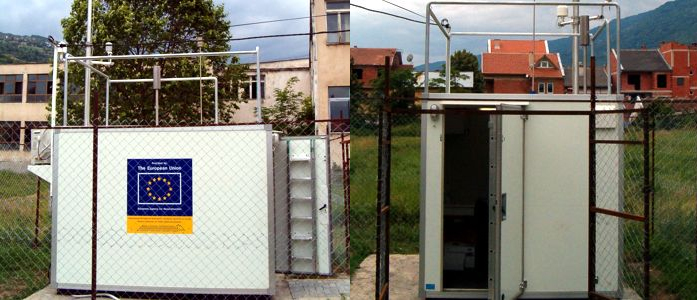
\includegraphics[width=1\textwidth]{figures/mernistanici.jpg}}
  \caption{Мерна станица за квалитет на воздухот во Тетово}
  \label{fig:titles}
\end{figure}

Податоците се мерат еднаш на секои 60 минути, и тие се испраќаат до сервер на \textbf{Министерството за Животна Средина и Просторно Планирање}, кои имаат задолжение да ги собираат, процесираат и складираат информациите доставени од станиците. Тие податоци се претставени на веб страната на министерството, каде што може да се види нивото на загаденост од секој тип на загадувач во размери кои се определени од Европската Унија~\cite{eulimits}.
\vspace{5mm}

Сепак, сајтот е прилично застарен, начинот на прикажување на податоците е збунивачки, и дефинитивно не е лесно преку мобилен уред да се пристапи до истите. Земајќи го сето тоа во предвид, заедно со актуелноста на темата во светски рамки, се одлучив на чекор што ќе го промени тоа, нарекувајќи го \textbf{МојВоздух}.

\section{Mотивација за дипломската работа}

Загаденоста на воздухот претставува многу битен фактор во нашиот живот. Секојдневно го гледаме, веќе и потсвесно, но дали навистина знаеме што дишеме?
\vspace{5mm}

Земајќи во предвид дека податоците за загаденоста на воздухот се достапни веќе од 2011 година, решив да ги искористам со цел подобро да се информирам себе си и останатите граѓани. Откривајќи дека не се достапни истите во отворен формат, и благодарение на предметот „Веб Базирани Системи“ каде што од д-р Димитар Трајанов и м-р Милош Јовановиќ научив многу за отворени податоци и семантички веб, одлучив не само да ги преземам и прикажам податоците на поинаков начин, туку истите да ги анотирам со веќе постоечка онтологија за тие да се достапни и до другите развивачи преку еден стандардизиран начин на пристап.

%%%%%%%%%%%%%%%%%%%%%%%
\chapter{Слични апликации}
При истражувањето кое што го направив за време на оваа дипломска, наидов на повеќе апликации од сличен карактер на МојВоздух. Секоја си имаше свои добри и лоши страни, и врз база на нив земав инспирација за креирање на тоа што денес е финален продукт.

\section{AirNow}
AirNow е вебсајт оддржуван од владата на САД, каде што го прикажуваат загадувањето на голем размер, т.е. врз поголеми области низ Америка. Тие не даваат податоци за мерења на одделни загадувачи, туку користат формула за пресметка на еден глобален индекс на загаденост земајќи ги сите загадувачи како фактори во него. Доброто нешто овде е што може да дадат предвидувања каква ќе биде загаденоста во наредните 24 часа, нешто што се пресметува врз база на претходно собрани податоци за тој период од годината.
\begin{figure}[H]
\centering
  \fbox{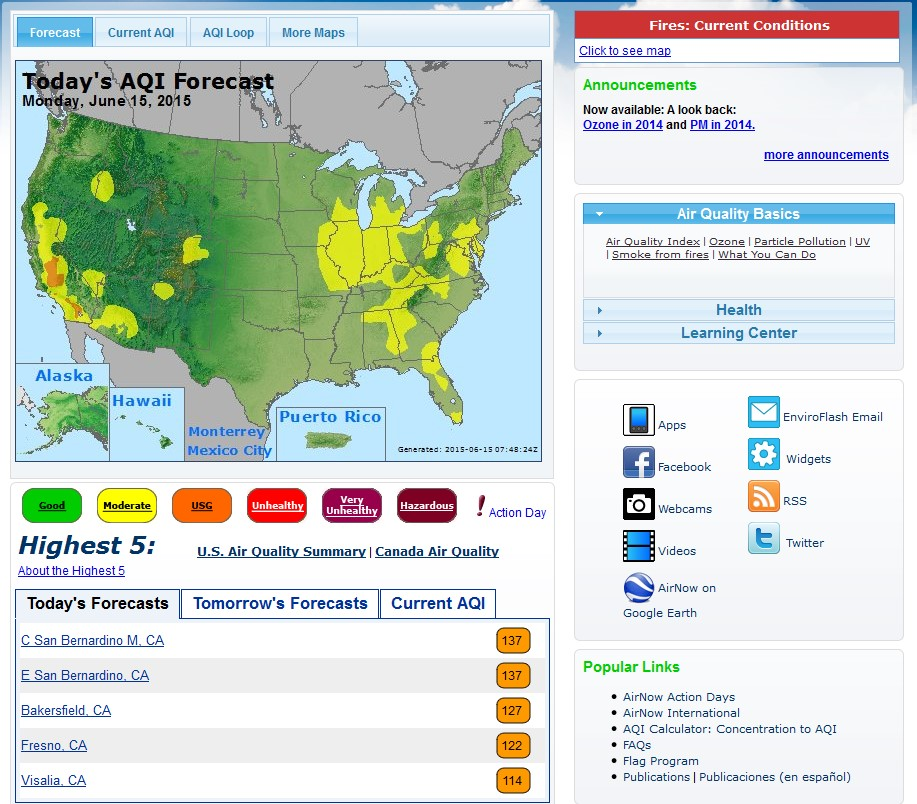
\includegraphics[width=0.7\textwidth]{figures/airnow.jpg}}
  \caption{AirNow}
  \label{fig:airnow}
\end{figure}

\section{Air Quality in Europe}
Оваа апликација е изработена од страна на Citeair фирмата, и покажува загаденост низ поголемите градови од ЕУ. За жал, таа веќе не е во функција од 2012 година, а соодветно добра замена во моментов нема.
\begin{figure}[H]
\centering
  \fbox{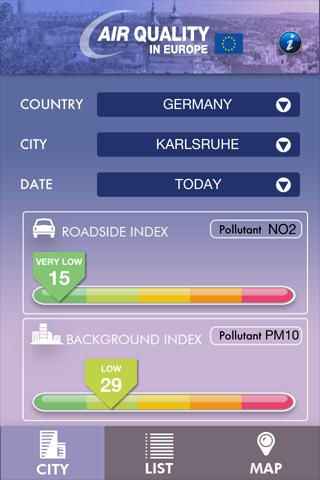
\includegraphics[width=0.5\textwidth]{figures/airqualityeu.jpg}}
  \caption{Air Quality in Europe}
  \label{fig:aireu}
\end{figure}
\vspace{5mm}

\section{Air Quality in China}
Кина е позната по големата загаденост во Шангај и Пекинг, и поради тоа имаат развиено апликација доста слична на AirNow, во која графички ги прикажуваат податоците за загаденост во двата најголеми градови во Кина. Во секој град има поставено повеќе мерни станици, и тие, исто како американците, пресметуваат и прикажуваат индекс на загаденост, но со можност за прегледување на загаденоста и од поединечни загадувачи.
\begin{figure}[H]
\centering
  \fbox{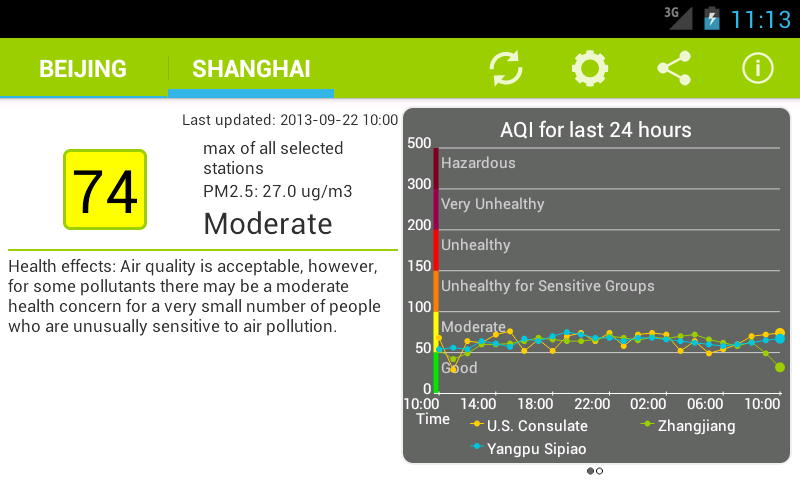
\includegraphics[width=0.7\textwidth]{figures/airqualitychina.png}}
  \caption{Air Quality China}
  \label{fig:airch}
\end{figure}

\section{BreezoMeter}
Како најдобра апликација од сите пронајдени беше Breezo Meter, апликација која што е достапна во САД и Израел, и користејќи ја софистицираната мрежа на мерни станици низ големите градови, може да прикаже heat-мапа во живо од загаденоста низ нив. За жал во Македонија имаме само 17 мерни станици, и анализа од ваков тип е доста тешка за да се изведе. Од дизајн аспект е многу добро сработена, што беше инспирација за мене да ја направам МојВоздух исто, ако не и подобра од нив.
\begin{figure}[H]
\centering
  \fbox{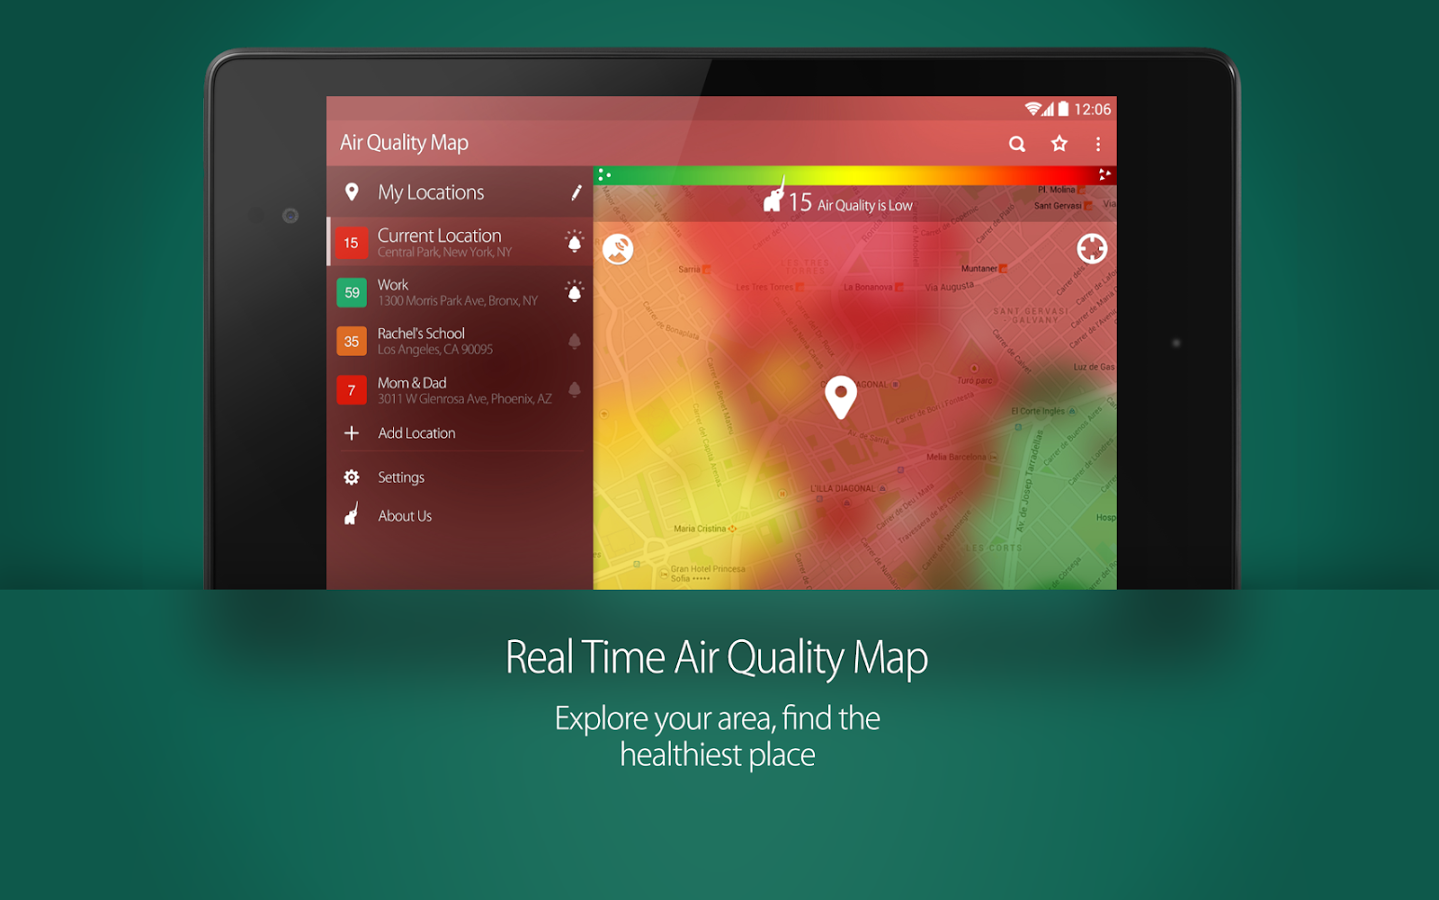
\includegraphics[width=0.9\textwidth]{figures/breezo.png}}
  \caption{Breezo Meter}
  \label{fig:breezo}
\end{figure}

%%%%%%%%%%%%%%%%%%%%%%%
\chapter{Податоци}
\section{Постоечкиот приказ на податоците}

На самиот почеток на моето истражување, барав да најдам како изгледа веќе постоечкиот приказ на податоците на сајтот на Министерството за Животна Средина и Просторно Планирање. 

\begin{figure}[H]
\centering
  \fbox{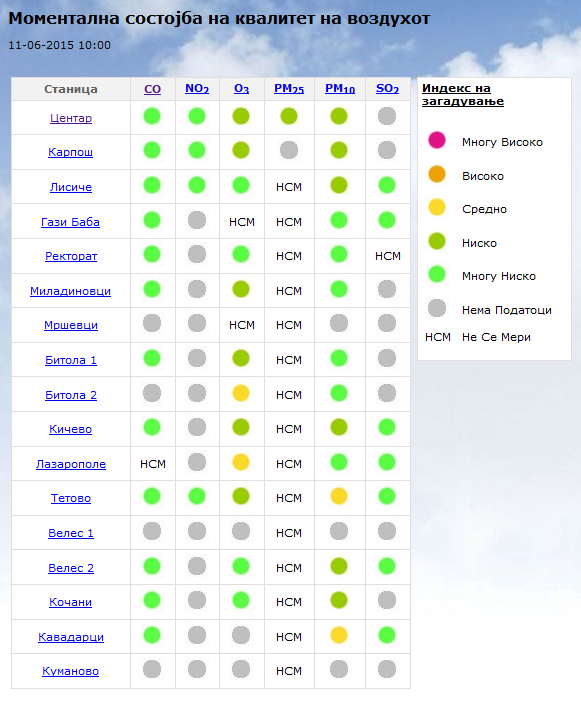
\includegraphics[width=0.5\textwidth]{figures/ministerstvo.png}}
  \caption{Сајтот на Министерството за Животна Средина и Просторно Планирање}
  \label{fig:ministerstvo}
\end{figure}

За жал, тие беа прикажани на многу застарен систем, во формат кој не е лесно разбирлив (поради сличноста на боите), и многу малку информации за деталните мерења. Секако, страната не беше прилагорена за работа од мобилен уред, и беше многу тешко истата од таму да се прегледа.
\vspace{5mm}

Доколку корисникот доволно добро ја загледа страната, ќе примети дека имињата на локациите на мерните станици, како и имињата на загадувачите, се всушност линкови кои водат до графичко претставување на мерењата. Овој чекор е доста неприроден за корисникот, а уште помалце воочлив.


\begin{figure}[H]
\centering
  \fbox{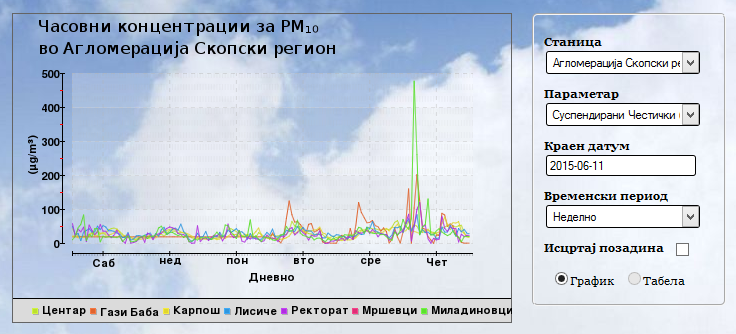
\includegraphics[width=1\textwidth]{figures/grafik.png}}
  \caption{Графички приказ на мерењата}
  \label{fig:grafik}
\end{figure}

Повторно, самиот график е доста не-иновативен, каде што тешко се читаат податоците поради нивното поклопување, како и лошиот избор на позадина. Преглед на истото преку мобилен уред е скоро и невозможно.


\section{Преземање на податоците}

При ирстражување кое го спроведов околу достапноста на податоците за загаденоста на воздухот, открив дека тие се дел од програмата на владата наречена Отворени Податоци. Преку таа програма може да се дојде до голем број на податоци со кои располагаат државните служби, и да се искористат во други проекти и цели. Меѓу тие податоци се наоѓаат и тие на министерерството.
\vspace{5mm}

За жал, податоците не се достапни ниту во полу структуриран, ниту во неструктуриран формат. На страната на проектот едноставно е поставен линк до сајтот на министерството. Тоа претставуваше пречка во првичното пронаоѓање на податоците, но го продолжив истражувањето, со чија помош ги пронајдов графиците на сајтот на министерството, и позадинскиот JSON кој им ги доставува мерките. 
\vspace{5mm}

За да се пристапи до податоците, треба да се искористи следното URL.
\vspace{5mm}

\begin{snippet}
\begin{verbatim}
http://airquality.moepp.gov.mk/graphs/site/pages/MakeGraph.php?graph=StationLineGraph
\end{verbatim}
\end{snippet}
\vspace{5mm}

На овој линк треба да се додадат наведените GET параметри за да се врати валиден JSON резултат.

\begin{itemize}
\item \textbf{station} - Име на станицата од која се преземаат податоците, пр. „SkopjeRegion“
\item \textbf{parameter} - Име на загадувачот за кој се преземаат податоците, пр. „CO“
\item \textbf{endDate} - Датумот на мерењето за кој се интересира, пр. „2014-12-22“
\item \textbf{timeMode} - Големината на податоците кои ќе ни се доставени, пр. дневни т.е. “Day„
\end{itemize}
\newpage
Доколку правилно се постават параметрите, податоците преку таа врска се добиваат во форматот прикажан на Слика~\ref{fig:jsonPodatoci}.

\begin{figure}[H]
\centering
\begin{snippet}
\begin{verbatim}
{"parameter":"CO",
    "measurements":{
        "20141222 00":{
            "Centar":"","GaziBaba":"1.33","Karpos":"1.83","Lisice":"1.40",
            "Rektorat":"1.48","Mrsevci":"","Miladinovci":"0.63"},
        "20141222 01":{
            "Centar":"","GaziBaba":"1.01","Karpos":"0.48","Lisice":"0.73",
            "Rektorat":"1.93","Mrsevci":"","Miladinovci":"0.45"},
        "20141222 02":{
            "Centar":"","GaziBaba":"0.73","Karpos":"0.59","Lisice":"1.14",
            "Rektorat":"1.07","Mrsevci":"","Miladinovci":"0.46"}
    }
}
\end{verbatim}
\end{snippet}
\caption{Извадок од JSON мерењата од сајтот на министерството}
\label{fig:jsonPodatoci}
\end{figure}
\vspace{5mm}

Во низата „measurements“ може да се пронајдат податоците од секоја мерна станица, а клучот на секој елемент од таа низа го претставува датумот и часот во кој што е направено мерењето, подесено во формат \textbf{YYYYMMDD HH}. Знаејќи ги имињата на сите 6 загадувачи и 17 мерни станици, може многу лесно да се пристапи до информации за секоја комбинација.

\section{Складирање на податоците}

Откако сите податоци ќе бидат прочитани и испарсирани, тие ги зачувувам во релациона база. На Слика~\ref{fig:basediagram} може да се види дизајнот на базата, кој е составен од 2 ентитети (локации и мерења), и една 1-N врска која го поврзува секое мерење со точно една дадена локација.

\begin{figure}[H]
  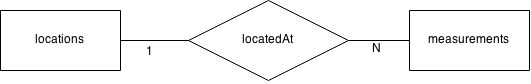
\includegraphics[width=1\textwidth]{figures/basediagram.png}
  \caption{ER диаграм за дизајн на релационата база}
  \label{fig:basediagram}
\end{figure}

Во секоја табела има повеќе полиња, прикажани на Слика~\ref{fig:bases}. Кај локациите освен идентификаторот, се чуваат и податоци за точната геограска локација на станицата, како и линк до DBPedia кој што ја објаснува истата. За секое мерење се чува локацијата каде што е направено, времето, колку е измерено, кој загадувач се мерел, знаменце кое означува колку е загадено местото, како и податоци за времето во дадениот момент кои се преземаат од друг сервис (температура, влажност на воздух, брзина на ветар и дали има во моментот врнежи).

\begin{figure}[H]
 \centering
  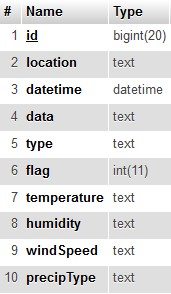
\includegraphics[width=0.25\textwidth]{figures/measurementbase.jpg}
  \hspace{5mm}
  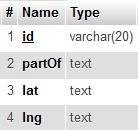
\includegraphics[width=0.25\textwidth]{figures/locationsbase.jpg}
  \caption{Изгледот на табелите measurements (лево) и locations (десно)}
  \label{fig:bases}
\end{figure}

Со помош на автоматизирана скрипта која се повикува на секој час, серверски се преземаат нови податоци и се складираат. Ова овозможува континуиран преглед на загадувањето, како и преглед во минатите денови кој е корисен за споредба и статистичка анализа.
\vspace{5mm}

%%%%%%%%%%%%%%%%%%%%%%%
\chapter{Изработка на веб сајт}
Поради потребата веќе-собраните податоци да се претстават на корисиницте во еден јасен и разбирлив формат, одлучив да изработам веб страна која што ќе е достапна на сите десктоп и мобилни уреди. На тој начин, сите корисници, независно од платформата која што ја поседуваат, ќе можат да ги прегледаат агрегираните и процесираните информации на брз и едноставен начин.
\section{Избор на технологија}
Со цел да се избере најпогодната технологија за изработка на овој дел од дипломската работа, се одлучив да го искористам PHP серверскиот јазик, кој е поддржан на сите серверски платформи и околини и лесно се вкопува со горе-споменатата MySQL база каде што се складирани податоците.

\vspace{5mm}

За корисничкиот дел, најсоодветното решение беше да се користи мој личен HTML изработен темплејт во кој ќе се вградат сите делови кои што се планирани, и истите лесно ќе се менливи. Поради малата природа на потребниот код, се одлучив да не користам веќе постоечки framework околини кои ќе одземат повеќе време за нивно подесување, него што ќе заштедат.
\section{Изработна на позадинскиот дел}
Серверскиот дел има три главни функции, и тоа да ги собира, складира и доделува податоците на апликацијата при нејзино барање. За таа цел, PHP серверскиот дел беше подигнат на веќе подесен сервер кој имаше поддршка за MySQL база и CornJobs кои ќе бидат објаснети подоле.
\vspace{5mm}

Самата PHP скрипта е составена од два дела, дел кој што ги собира и складира информациите, и дел кој што ги доставува на апликацијата врз база на дадени параметри. 

\subsection{Преземање и складирање на податоците}
Првиот се поврзува на сајтот на министерството со секоја комбинација на параметри (локации на мерни станици и параметри, т.е. загадувачи). Пример за ова поврзување е даден во прилог.

\vspace{5mm}

\begin{snippet}
\begin{verbatim}
http://airquality.moepp.gov.mk/graphs/site/pages/MakeGraph.php?graph=StationLineGraph
                                &station=SkopjeRegion&parameter=PM10&endDate=06-06-2015&timeMode=Day
\end{verbatim}
\end{snippet}
\vspace{5mm}

До податоците се пристапува на начин објаснет во Глава 2. Откако ќе се пристапи до нив, се парсира JSON одговорот. За секоја локација одделно се преземаат и временските услови во моментот на мерење, поточно влажноста на воздухот, температурата, брзината на ветрот и дали врне во дадениот момент. Овие податоци се преземаат од јавно достапно API на сервисот \textbf{Forecast.io}. На нивниот endpoint се препраќаат географските координати на мерната станица што во дадениот момент се проверува, и повратно се добива повторно JSON одговор кој се парсира. На Слика ~\ref{fig:preudocode} може да се види псевдо код кој покажува како се извршува преземањето и складирањето на податоците од сајтот на министерството и сајтот на Forcast.io.


\begin{figure}[H]
\centering
\begin{snippet}
\begin{verbatim}
    foreach(location in StationLocations){
        getLocationMeasurements();
        if(location in SkopjeLocations && skopjeWeather not present){
            getWeather(location.lat, location.lng);
        }
        else if(location not in SkopjeLocations){
            getLocationWeather(location.lat, location.lng);
        }
        storeInformationInDB();
    }
\end{verbatim}
\end{snippet}
\caption{Псевдо-код за преземање и зачувување на податоците}
\label{fig:preudocode}
\end{figure}

Бидеjќи податоците на сајтот на министерството се обновуваат секој час, на серверот каде што е поставен позадинскиот дел, подесена е \textbf{CornJob} скрипта. Нејзината намена е да ја повикува PHP скрипта за преземање на податоците на даден интервал, т.е. во нашиот случај, на секој час.
\vspace{5mm}

Еден од проблемите на кој што наидов беше дека различни мерни станици доставуваат податоци во различна минута од часот, додека некои станици ги доставуваат податоците дури и час и половина откако се измерени. За да се избегне овој проблем, и да се задржи конзистентноста, скриптата ги повлекува податоците со доцнење од еден час и половина, за да се осигура дека сите станици веќе имаат измерено и доставено податоци до серверот на министерството.

\subsection{Предавање на податоците}

Вториот од двата PHP дела е тој кој што ги предава податоците на корсничкиот дел од апликацијата кога тоа ќе биде побарано од него. За таа цел, изработив посебна PHP скрипта која што служи како API крајна цел, и кога до неа ќе бидат испратени сет параметри, таа соодветно гради SQL прашалник со кој презема податоци од базата, ги претвара во JSON формат, и истиот го враќа на апликацијата, мобилна или веб.
\vspace{5mm}

Параметрите до скриптата се предаваат преку GET повик, и може да се препратат следните:

\begin{itemize}
\item \textbf{last20days} - Ги враќа податоците за последните 20 дена
\item \textbf{date} - Ги враќа точните податоци за даден датум
\item \textbf{hour} - Ги враќа податоците за точниот час (мора да се користи заедно со \textbf{date}
\item \textbf{last24} - Ги враќа податоците за последните 24 часа (не може да се користи со сите претходни или со \textbf{last}
\item \textbf{last} - Го враќа само последниот измерен податок (не може да се корисни со сите претходни)
\item \textbf{type} (опционален) - Ги враќа податоците за точно тој тип на мерење
\item \textbf{location} (опционален) - Ги враќа податоците за точно таа мерна станица
\end{itemize}
\vspace{5mm}

Пример за URL кое што се повикува од некоја од апликациите:
\vspace{5mm}

\begin{snippet}
\begin{verbatim}
http://gorjan.rocks/clients/airquality/returnNewData.php?last24&location=Centar&type=PM10
\end{verbatim}
\end{snippet}
\vspace{5mm}


Одговорот во JSON формат, низа на мерења, се добива во следниот формат:


\begin{figure}[H]
\centering
\begin{snippet}
\begin{verbatim}
[
    {"id":"420253","location":"Centar","datetime":"2015-06-13 18:00:00","data":"30.91",
    "type":"PM10","flag":"1","temperature":"27.66","humidity":"0.3","windSpeed":"1.01",
    "precipType":"rain"},
    {"id":"420149","location":"Centar","datetime":"2015-06-13 17:00:00","data":"29.45",
    "type":"PM10","flag":"1","temperature":"27.9","humidity":"0.35","windSpeed":"0.97",
    "precipType":"rain"},
    {"id":"420045","location":"Centar","datetime":"2015-06-13 16:00:00","data":"25.70",
    "type":"PM10","flag":"1","temperature":"30.61","humidity":"0.29","windSpeed":"0.64",
    "precipType":"rain"}
    ...
]
\end{verbatim}
\end{snippet}
\caption{JSON одговор од серверот}
\label{fig:jsonPodatociOdgovor}
\end{figure}



\section{Изработка на корисничкиот дел}

Корисничкиот дел беше наменет да е јасен, читлив, разбирлив и пред се, едноставен за употреба. Бидејќи целтана група на корисници е доста голема, решив да го искористам \textbf{Google Material}~\cite{googlemat} дизајн стандардот, и користејќи ги неговите компоненти, да го дизајнирам веб интерфејстор за корисниците.
\vspace{5mm}


Главната дизајн компонента на апликацијата е кругот кој се полни и менува боја во зависност од загаденоста во околината. Колку е таа поголема, толку повеќе се исполнува периметарот на кругот, и бојата прелева од зелена - означувајќи чист воздух, преку жолта - означувајќи делумно загаден воздух, до црвена - означувајќи големо загадување на воздухот. Во моментот кога кругот ќе се испонли, значи дека загадувањето ја надминало и највисоката граница за тој тип загадување поставена од Европската Унија. Во центарот на гругот е испишана мерката, и мерната единица за истата. Ова е прикажано на Слика~\ref{fig:krug}.
\vspace{5mm}


\begin{figure}[H]
\centering
  \fbox{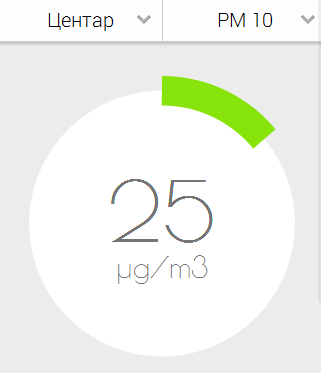
\includegraphics[width=0.4\textwidth]{figures/krug.png}}
  \caption{Главната дизајн компонента: кругот}
  \label{fig:krug}
\end{figure}

Следно беа елементите наречени „карти“. Тие се мали целини на податоци кои прикажуваат информации независно од другите карти околу нив, но сепак во ист контект. За ова да биде појасно, во овој случај секоја картичка ја добива информацијата за тоа колку е загаден воздухот, и со таа информација покажува различни информации, од тоа колку дена до сега бил чист возухот, што точно е овој тип на загадување и кој го предизвикува. 
\vspace{5mm}


\begin{figure}[H]
\centering
  \fbox{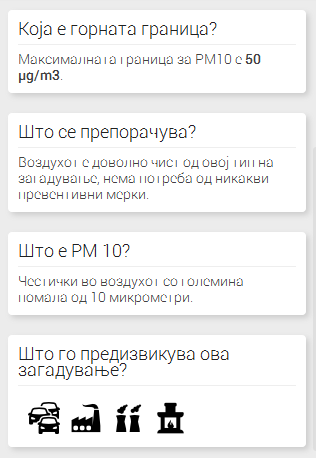
\includegraphics[width=0.4\textwidth]{figures/cards.png}}
  \caption{Информативни картички}
  \label{fig:cards}
\end{figure}
\vspace{5mm}


Друг битен дел за корсникот е графичкото претставување на собратните податоци. Со помош на ваквиот приказ, може детално да се види движењето на загадувањето по денови. За да се постигне ова, од позадинскиот дел се повлекуваат податоците за последните 9 дена од одбраната локација и тип на загадувач, и истите се проследуваат до функцијата за исцртување на графикот. 
\vspace{5mm}

За време за прикажување на веб верзијата на корисници, дел од нив се заинтересираа за можноста за статичка одбработка на податоците кои што се собрани во базата. Имајќи го тоа во предвид, во мобилната апликација овој модул е доста проширен со многу повеќе податоци како временските услови на локацијата во моментот на мерењето, на кој ден од неделата е направено тоа мерење, и дали тој ден бил работен или неработен. Значајноста на сите овие податоци е прикажана во следната глава каде што во повеќе детали се објаснува за изработката на мобилната апликација.

\begin{figure}[H]
\centering
  \fbox{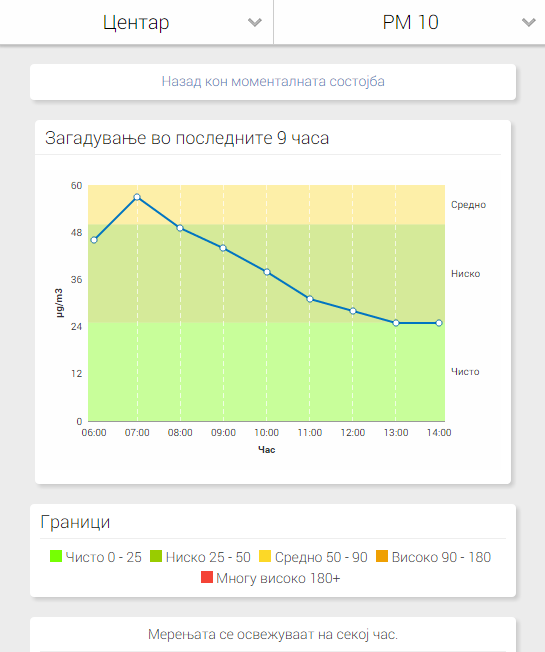
\includegraphics[width=0.8\textwidth]{figures/graf.png}}
  \caption{Загадувањето во последните 9 дена}
  \label{fig:graf}
\end{figure}

Бидејќи МојВоздух започна со креирањето на веб апликацијата, таа во моментов има помалку можности за разлика од нејзината сестринска апликација на Android оперативниот систем. Причините за ова се објаснети во следната глава. Сепак, веб верзијата беше лесна за градење на брз прототип од идеите и прикажување на истиот на поголема публика со цел добивање критики. Имајќи ги сите тие на едно место, започнав со креирање на мобилната апликација, која што беше наменета на Android системот.

%%%%%%%%%%%%%%%%%%%%%%%
\chapter{Изработка на мобилна апликација}
После собраните критики за веб верзијата на МојВоздух, решив да изработам native мобилна апликација користејќи ги истите податоци како и во претходната. Се решив на овој чекор од повеќе причини. Брзината на работа на апликациите на телефон сеуште ја надмиува таа на веб апликациите. При неколкукратни мерења, времето на стартување на мобилната апликација беше знемарливо мало во споредба со отварање на прелистувачот, внесување на адресата на страната и чекање таа да се вчита.


\section{Избор на технологија}

Во изборот на технологијата играа повеќе фактори:

\begin{itemize}
\item Потребното време за изработка
\item Досегашното искуство со платформата
\item Користеноста на платформата во целната група
\end{itemize}

Гледајќи од сите овие фактори, потребното време за изработка е еднакво на скоро сите три платформи поради нивната развиеност до одреден степен на целосна прифатеност од производителите на мобилните уреди. Но тој фактор директно зависи од следниот, т.е. досегашното мое искуство со програмирање на овие платформи. На iOS немав никаква можност да програмирам до овој момент, за разлика од проектите кои ги имам работено на Android и Windows Phone. Заедно со тој податок, остана третиот фактор, кој е и најзначаен меѓу сите, а тоа е користеноста на платформата во целната група. Сепак апликацијата е наменета да биде користена од страна на што е можно повеќе корисници, и моето досегашно искуство и знаење може да се прилагоди за да ги задоволи овие потреби. 
\vspace{5mm}


Врз база на претходни мерења на мобилната страна на МојВоздух, статистиките покажаа дека повеќе од 80\% посетителите доаѓаат од мобилен уред~\cite{mobusers}, а од нив повторно 80\% се на Android оперативниот систем. Тоа беше главна причина да започнам со развој и на Android мобилна апликација, за да го задоволам тој пазар на мобилни посетители.

\section{Изработна на позадинскиот дел}

Посебна изработка на позадинскиот дел нема, бидејќи се користи истиот што го користи и веб верзијата на МојВоздух. Со истите повици се добиваат истите податоци во JSON формат, кои се парсираат и соодветно прикажуваат на корисникот. Поголем труд вложив во корисничкиот дел каде што се прикажуваат податоците слично на тоа како во веб верзијата, но со поголем број на опции.

\section{Изработка на корисничкиот дел}

За изработка на корисничкиот дел, беше потребно да изберам работна околина. Земајќи го фактот дека на почетокот на проектот, Android Studio како околина беше сеуште во бета фаза на развојот, и не беше стабилна за изработка на апликации за широка употреба, решив да го користам постарото решение, т.е. Eclipse околината.
\vspace{5mm}


\begin{figure}[H]
\centering
  \fbox{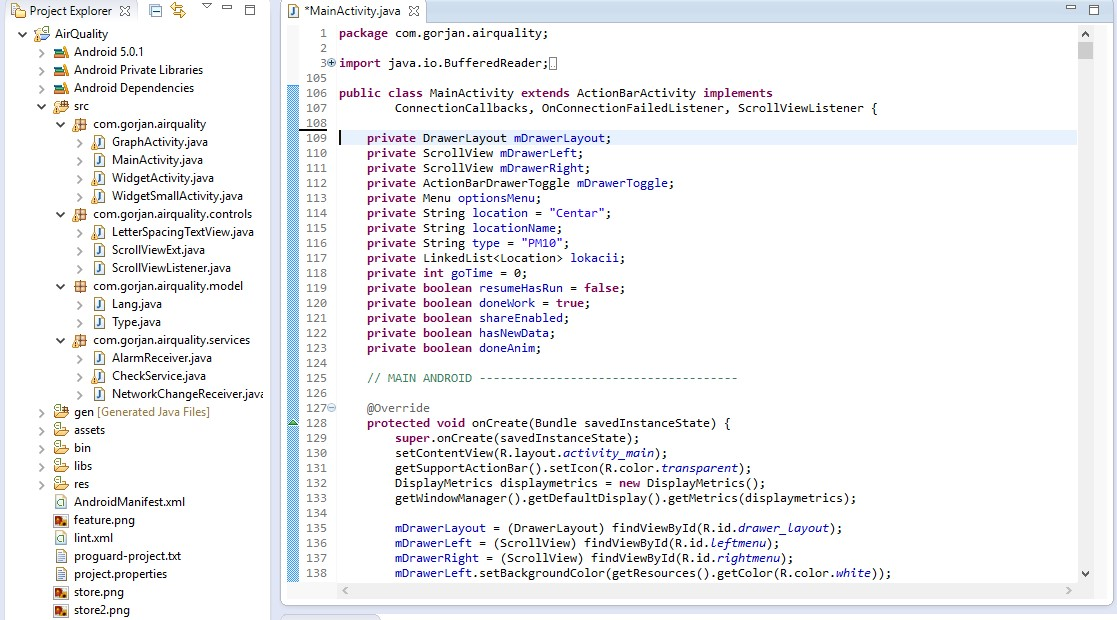
\includegraphics[width=0.985\textwidth]{figures/eclipse.jpg}}
  \caption{Изгледот на работната околина во Ecplise}
  \label{fig:ecplise}
\end{figure}

\vspace{5mm}

Проектот е поделен во 2 сектори, секој од нив детално објаснет во продолжение.

\newpage
\subsection{Видливи делови}

Главните делови на самата апликација се напишани овде, а тоа се 4: основниот екран, екранот за графички приказ и двата вида на виџети кои коирсникот може да ги постави на работната површина на мобилниот уред.


\begin{figure}[H]
\centering
  \fbox{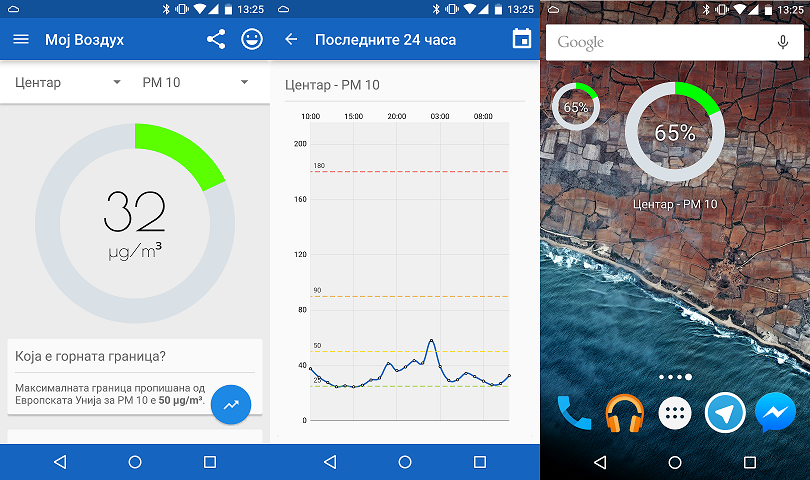
\includegraphics[width=0.985\textwidth]{figures/mojvozduh.png}}
  \caption{Главните видливи екрани}
  \label{fig:mainpage}
\end{figure}

Почетниот екран што го гледа корисникот кога ќе ја подигне апликацијта е најбитен од сите, и мора да остави добар впечаток за корисникот повторно да се наврати на истата апликација. 
\vspace{5mm}

\subsubsection{Почетен екран}

Најгоре се смеснтени листа на мерни станици, и листа на загадувачи кои се достапни за одбраната мерна станица. Под нив доаѓа главниот круг на апликацијата што беше објаснет во секцијата за веб апликацијата. Понатаму доаѓаат секции што кажуваат која е горната граница за одбраното загадување пропишана од ЕУ стандарди, број на денови до овој момент во кои просекот на загадувањето не ја надминал границата на нормала (доколку тоа се деси, бројачот се ресетира), објаснување што е одбраниот тип на загадување, кој го предизвикува и што се препорачува земајќи ја во предвид моменталната измерена состојба.
\vspace{5mm}


\subsubsection{Екран со графички приказ}
Со одбирање на копчето за графички приказ во долниот десен ќош на главниот екран, се прикажува следниот екран на кој е поставен график. Овој график може да прикаже податоци за веќе одбраното загадување и локација од претходниот екран, и тоа за последните 24 часа или последните 20 дена. Со одбирање на некоја од точките на графикот се прикажуваат повеќе информации за даденото мерење, како тогашната температура, влажност на воздухот, брзина на ветарот и дали во моментот врнело. Сите овие податоци допринесуваат до можноста за статистичка анализа на добиените мерења, преку која ќе може да се согледаат кои услови влијаат врз зголемување на загадувањето.


\subsubsection{Виџети}

Виџетите се начин на корисникот брзо го прегледа загадувањето на работната површина од неговиот телефон, без притоа да треба да ја отвори апликацијата. Поради големиот број мобилни со различна  големина на екран достапни на пазарот, потребно беше да се направат две варијанти од виџетот: поголема, што зафаќа поголем простор и ја прикажува мерната странициа и загадувањето, како и помала, која што само го прикажува кругот и процентуалното загадување. Овие виџети се испрограмирани за кога ќе се надмине дозволеното загадување, од проценти да се претворат прикажаните податоци во број на пати. Така, мерење од „150\%“ ќе стане „х1.5“, заштедувајќи на простор и олеснувајќи го читањето.

\subsubsection{Изменети контроли}

Двете изменети контроли кои што се користат во проектот се изменет ScrollView, и изменет TextView. Причината за промените на овие две контроли е за да се даде подобро корисничко искуство. Со помош на првата, може да детектираме кога корисникот на главниот екран стигнал до дното на листата од карти, и тогаш можеме копчето за повикување на екранот за график да го направиме проѕирно, со цел да не поклопува дел од текстот под него. Со втората компонента може да ја направиме од естетски аспект поубава картата која прикажува колку денови имало чист воздух до сега, т.е. да може лесно да го подесуваме просторот помеѓу буквите (ствојство кое не доаѓа само по себе во Android околината).

\begin{figure}[H]
\centering
  \fbox{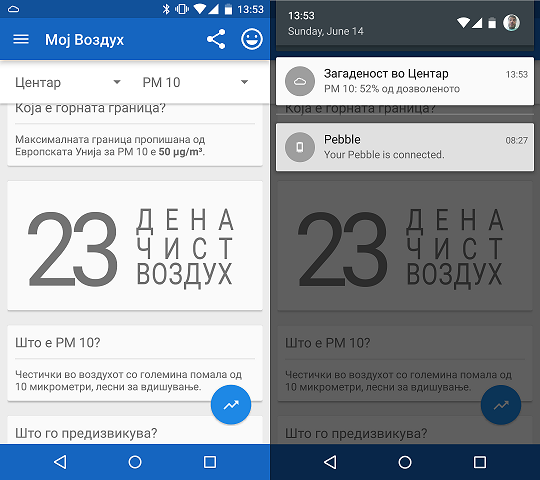
\includegraphics[width=0.9\textwidth]{figures/controls.png}}
  \caption{Друг поглед на апликацијата}
  \label{fig:controls}
\end{figure}


\subsubsection{Додатни можности}
Како додатни можности се вбројуваат следните:
\begin{itemize}
\item Опција за смена на јазик (моментално Македоснки и Англиски).
\item Опција за постојано известување/нотификација на телефонот. за загаденоста (видливо на Слика~\ref{fig:controls}).
\item Опција за постојано следење на локацијата и прилагодување на известувањето за најблиската мерна станица до корисникот.
\item Опција за прикажување на совети за заштита на воздухот преку корисење на јавен транспорт и велосипеди.
\item Опција за споделувања на сегашното загадување преку слика на социјалните мрежи.
\end{itemize}


\subsection{Позадински сервиси}
Позадинските сервиси се наменети да ја и доставуваат најнови податоци на апликацијата. Тие се подесени така да на секој час, се поврзат со позадинскиот дел на серверот, и повлечат нови информации за загадувањата. Истите информации се потоа зачувани локално на уредот и не е потребна интернет конекција за нивно прегледување. Бидејќи за оваа операција да е успешна, потребно е да има активна интернет конекција, и се додека таа не се воспостави, апликацијата нема да праќа нови барања кон серверот.


%%%%%%%%%%%%%%%%%%%%%%%
\chapter{Влијание на МојВоздух врз корисниците}
Во 2011 година, кога за прв пат се поставија сензорите и информативните табли за загаденоста на воздухот, се формираше граѓнско движење кое алармираше за високото ниво на честички во атмоферата. За жал, ништо не се превзема, и движењето се смири, како сите да заборавија на проблемот кој постојано е присутен. Главната цел на МојВоздух беше да го врати назад вниманието врз овој проблем, бидејќи тој сеуште постои и не е решен. 
\vspace{5mm}

Во првиот месец одкако МојВоздух беше објавен, воздухот во Тетово доситгна рекордно висока загаденост, 20 пати над максимално дозволениот лимит пропишан од ЕУ. За да го искажат својот гнев, граѓаните на Тетово, Гостивар и Скопје, како својат профилна слика на социјалните мрежи го поставија познатиот круг од МојВоздух.

\begin{figure}[H]
\centering
  \fbox{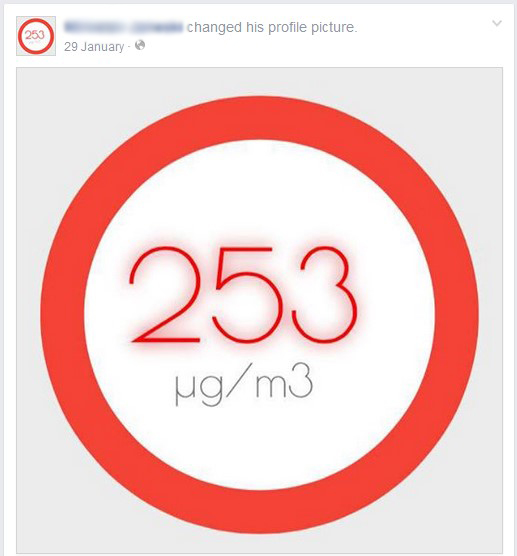
\includegraphics[width=0.6\textwidth]{figures/fbprofile.jpg}}
  \caption{Друг поглед на апликацијата}
  \label{fig:fbprofile}
\end{figure}

Друг начин преку кој што МојВоздух имаше влијание врз корисниците беше кога се организираше на протестот за загаден воздух во Скопје \cite{protest}. Иако не беше директно влучен во протестот, верувам дека со самото медиумско изложување и зголемената популарност на апликацијата, придонесе до формирање на едно вакво движење кое ја има истата цел како и апликацијата.

\begin{figure}[H]
\centering
  \fbox{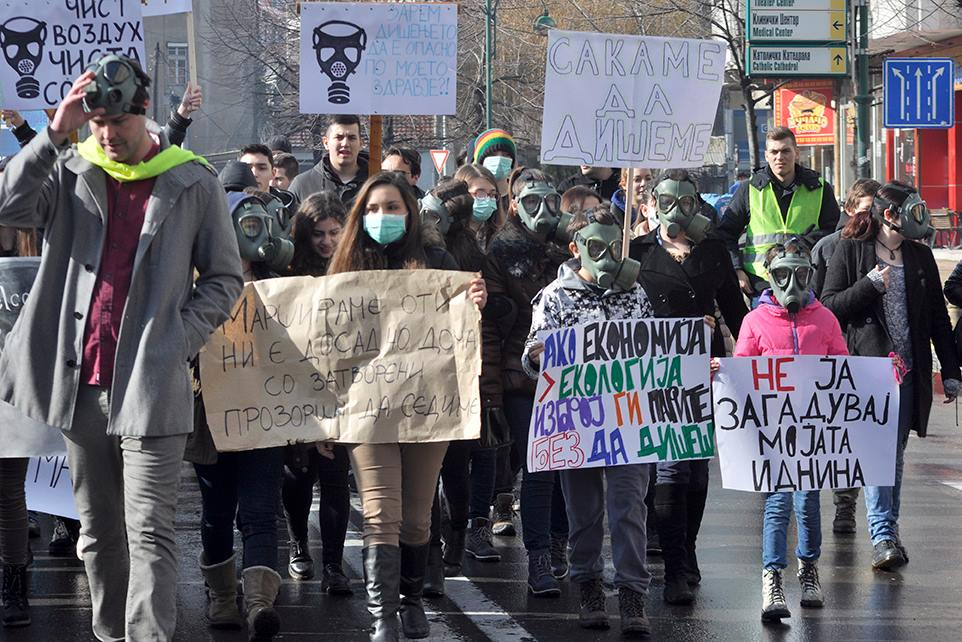
\includegraphics[width=0.9\textwidth]{figures/protest.jpg}}
  \caption{Друг поглед на апликацијата}
  \label{fig:protest}
\end{figure}
%%%%%%%%%%%%%%%%%%%%%%%
\chapter{Одбирање соодветна онтологија}

Една од целлите на оваа дипломска работа работа беше да сите овие мерења ги мапирам на D2RQ база со соодветни онтологии, а потоа да бидат достапни преку SPARQL интерфејсот кој е вграден во D2RQ. Како објаснение, D2RQ претставува серверска апликација која што претвара веќе постоечка релациона база во множество на податоци до кое може да се пристапи преку SPARQL јазикот, и истите да се претстават во соодветен RDF формат, како поврзани податоци.
\vspace{5mm}


За тоа да се постигне, требаше да пронајдам соодветна онтологија која што се занимава со мерења на загадување на воздухот. Тоа се покажа како доста тешка задача. Најпрвин ја разгледав \textbf{Sematic Sensor Network онтологијата} развиена од W3C, но таа се покажа како малку корисна. Сепак, со помош на подолго истражување заедно со менторот Трајанов, успешно пронајдовме таква онтологија, која се нарекува \textbf{PescadoData}.

\section{Pescado онтологија}

Развиена од страна на Data \& Knowledge Management истражувачката група која е дел од Информациско Технолошкиот Центар во Fondazione Bruno Kessler, \textbf{Pescado онтологијата} се занимава точно со мапирање на податоци за мерења на PM10, PM2.5, CO и други загадувачи во воздухот, како и временски услови што во нашиот случај најдоа додатна примена.
\vspace{5mm}

По проучување на онтологијата, се одлучив да ги искористам следните класи при анотирање на нашите податоци.

\begin{itemize}
\item \textbf{pescadoData:HumidityValue} - Анотирање на влажноста на воздухот 
\item \textbf{pescadoData:TemperatureValue} - Анотирање на температурата на воздухот
\item \textbf{pescadoData:WindSpeedValue} - Анотирање на брзината на ветрот
\end{itemize}

За подобро анотирање на секое мерење, се одлучивме тие да ги поделиме, и секој тип на загадувач да го анотираме со класа од сопствениот тип. Во Pescado онтологијата постојат точен број на класи кои соодветствуваат со нашите мерења.

\begin{itemize}
\item \textbf{pescadoData:PM10IndexValue}
\item \textbf{pescadoData:PM2.5IndexValue}
\item \textbf{pescadoData:COIndexValue}
\item \textbf{pescadoData:NO2IndexValue}
\item \textbf{pescadoData:SO2IndexValue}
\item \textbf{pescadoData:O3IndexValue}
\end{itemize}


\section{Geo онтологија}

\textbf{Geo онтологијата}, која што е една од основните онтологии, помогна за мапирање на географските позиции на мерните станици. Имајќи ги точните GPS координати на секоја станица, ги искористив следните анотирања.

\begin{itemize}
\item \textbf{geo:location} - Послужи за rdf:type на локациите на мерните станици
\item \textbf{geo:lat} - Географска ширина
\item \textbf{geo:lng} - Географска должина
\end{itemize}

\section{DBPedia-Owl}

За да може да се поврзат локациите со конкретни градови кои се поставени како ресурси на DBPedia, ја искористив \textbf{DBPedia-Owl онтологијата}.

\begin{itemize}
\item \textbf{dbpedia-owl:isPartOf} - Object-type property кој ја поврзува локацијата со ресурс од DBPedia
\end{itemize}

\section{Prov онтологија}

\textbf{Prov онтологијата}, развиена од W3C, ни послужи за анотирање на локацијата каде што е направено мерењето, како и времето на генерирање на податоците.

\begin{itemize}
\item \textbf{prov:atLocation} - Локација на мерната станица
\item \textbf{prov:generatedAtTime} - Време на генерирање на податоците
\end{itemize}

%%%%%%%%%%%%%%%%%%%%%%%
\chapter{Мапирање на податоците во D2RQ}

\section{Инсталација и подесување на D2RQ}

Инсталацијата на D2RQ не престставува голема компликацијата. Со неговото преземање од инсталациониот сервер, распакување во локален директориум на серверот, и подигнување со следната команда се доволни за работа на D2RQ (секако серверот се подигнува откако ќе се изгенерира мапирањето, нешто што е објаснето во следната секција).

\begin{figure}[H]
\centering
\begin{snippet}
\begin{verbatim}
d2r-server [--port port] [-b serverBaseURI] [--fast] [--verbose] [--debug] mapping-file.ttl
\end{verbatim}
\end{snippet}
\caption{Команда за подигнување на D2RQ сервер}
\label{fig:d2rqrun}
\end{figure}

Секоја од командите која што се наоѓа во средни загради значи дека не е задолжителна за стартување на серверот. Во продолжение се дадени објаснувања за сите нив:

\begin{itemize}
\item \textbf{d2r-server} - Извршната програма на серверот.
\item \textbf{--port} - Портата на која да се подигне серверот, основната е 2020.
\item \textbf{-b} - Основно URL каде ќе биде стартуван серверот, за да работат правилно линковите во него. Пример ако серверот по стартувањето ќе може да се пристапи на http://gorjan.rocks:2020, тогаш тоа треба да се постави како основно URL.
\item \textbf{--fast} - Овозможува специјални оптимизации за брзина на лоадирање на податоците од база, и се препорачува да се користи се додека не се забележат проблеми.
\item \textbf{--verbose} - На излез се појавуваат повеќе информации околу подигнување на серверот.
\item \textbf{--debug} - На излез се појавуваат многу повеќе информации околу подигнување на серверот. 
\item \textbf{mapping-file.ttl} - Фајлот што сме го изгенерирале како мапирање на постоечките податоци, и ќе се користи како упатство на серверот за пристап до истите.
\end{itemize}

Сите овие конфигурации може да се додадат и во мапирачкиот фајл за да се оселни нивното менување и конзистентност. Пример за такви подесувања додадени на врвот на мапирачкиот фајл се следни. Може да се забележи дека повеќе подесувања се достапни на овој начин за разлика од претходниот.

\begin{figure}[H]
\centering
\begin{snippet}
\begin{verbatim}
<> a d2r:Server;
  rdfs:label "Air Pollution Macedonia - D2RQ";
  d2r:baseURI <http://gorjan.rocks:2020/>;
  d2r:port 2020;
  
  d2r:sparqlTimeout 300;
  d2r:pageTimeout 5;

  d2r:limitPerPropertyBridge 20;
  d2r:limitPerClassMap 20;

  meta:datasetTitle "Air Pollutant Mesurements";
  meta:datasetDescription "Measurements from 17 stations in Macedonia for 6 types of pollutants." ;
.
\end{verbatim}
\end{snippet}
\caption{Пример RDF конфигурациона датотека}
\label{fig:conf}
\end{figure}

Претходно необјаснетите параметри се објаснети во продолжение.

\begin{itemize}
\item \textbf{label} - Име на серверот, стандарден RDFS таг.
\item \textbf{sparqlTimeout} - Времето по кое што серверот ќе се откаже од одбработка на SPARQL команда.
\item \textbf{pageTimeout} - Времето по кое што серверот ќе се откаже од прикажување на некоја страна.
\item \textbf{limitPerPropertyBridge} - Лимит на бројот на врски меѓу ентитети прикажани на веб верзијата. Може да ја зголеми брзината на работата на серверот, но тогаш преку веб верзијата нема да може да се пристапи до сите податоци (ќе мора да се користи SPARQL прашалник.
\item \textbf{limitPerClassMap} - Лимит на бројот на ентитети прикажани на веб верзијата. Може да ја зголеми брзината на работата на серверот, но тогаш преку веб верзијата нема да може да се пристапи до сите податоци (ќе мора да се користи SPARQL прашалник.
\item \textbf{datasetTitle} - Наслов на сетот на податоци прикажани преку серверот.
\item \textbf{datasetDescription} - Опис на сетот на податоци прикажани преку серверот.

\end{itemize}



\section{Генерирање и подесување на мапирањето}

Откако ќе се инсталира D2RQ платформата, таа мора да се поврзе со нашата постоечка база на податоци, и соодветно да се мапираат колоните во базата со анотациите одбрани од онтологиите наведени погоре.
\vspace{5mm}

Најпрво треба да се генерира почетно мапирање кое после ќе се модификува. Тоа се прави со веќе вграденатата алатака во D2RQ, која на влез ги прима податоците за најава во базата, а на излез генерира \textbf{TTL (Turtle)} датотека која ги содржи сите потребни мапирања за да се покрене серверот. Командата која што се повикува за ова да се изврши е прикажана на Слика~\ref{fig:pocetnoMapiranje}.

\begin{figure}[H]
\centering
\begin{snippet}
\begin{verbatim}
generate-mapping -o mapping.ttl -d driver.class.name -u db-user -p db-password jdbc:url:...
\end{verbatim}
\end{snippet}
\caption{Команда за генерирање на почетно мапирање}
\label{fig:pocetnoMapiranje}
\end{figure}
\vspace{5mm}

Откако ќе се генерира почетното мапирање, треба да се проучат резултатите и да се модифирираат соодветно. Но тука наидов на проблем: Немаше генерална класа „мерење“ што можевме да ја доделиме на табелата measurements како нејзин тип, туку како што беше наведено погоре, постојат само класи за секој тип на мерење одделно. За да се реши овој проблем, самиот D2RQ јазик за мапирање има опција да задава услови, т.е. да генерира класа само ако е задоволен некој услов од податоците. Тоа го искористив, давајќи го условот да типот на мерењето мора да е од истиот тип кој што се задава во класата. Така можев секој тип на мерење да го одделиме во сопствена класа, а едно од тие одделувања е прикажано на Слика~\ref{fig:pm10merenje}.

\begin{figure}[H]
\centering
\begin{snippet}
\begin{verbatim}
# Table measurements PM10
map:measurementsPM10 a d2rq:ClassMap;
	d2rq:dataStorage map:database;
	d2rq:uriPattern "measurements/@@measurements.id@@";
	d2rq:class pescadoData:PM10IndexValue;		
    d2rq:condition "measurements.type = 'PM10'";
    d2rq:condition "measurements.data != ''";
	d2rq:classDefinitionLabel "measurementsPM10";
	.
\end{verbatim}
\end{snippet}
\caption{Модифицирано мапирање за мерења на PM10 честички}
\label{fig:pm10merenje}
\end{figure}

Објаснување за подесувањето во мапирачкиот фајл е дадено во продолжение.

\begin{itemize}
\item \textbf{dataStorage} - Локацијата од каде да се повлекуваат податоците.
\item \textbf{uriPattern} - Клучот по кои ќе се идентификуваат сите редици од оваа табела.
\item \textbf{class} - Класата од избраната онтологија која ќе соодветствува на ова мапирање. Бидејќи класите од Pescado се специфички за секое мерење, следното подесување се грижи да ова се само PM10 мерења.
\item \textbf{condition} - Со помош на ова подесување може да се даваат услови да само одредени редици од табелата го добијат ова мапирање. Во примерот ограничуваме да колоната 'type' има вредност 'PM10', а колоната 'data' да не е празна.
\item \textbf{classDefinitionLabel} - Наслов на мапирањето.

\end{itemize}

%%%%%%%%%%%%%%%%%%%%%%%
\chapter{Корисни SPARQL прашалници}

Во прилог се дел од можните корисни прашалници преку кои може да се пристапи до информациите сместени во базата. Така анотирани, може да се извлечат доста корисни статистики, а преку поврзување со други податочни сетови, како DBPedia, може да се дополнат веќе постоечките информации со нови и еднакво корисни.

\begin{figure}[H]
\centering
\begin{snippet}
\begin{verbatim}
SELECT DISTINCT ?loc ?date ?value WHERE {
  ?s rdf:type pescadoData:PM10IndexValue;
  rdf:value ?value;
  prov:atLocation ?loc;
  prov:generatedAtTime ?date.
}
ORDER BY DESC(?date)
LIMIT 100
\end{verbatim}
\end{snippet}
\caption{Преземање на последните 100 мерења за PM10 од сите станици}
\end{figure}

\begin{figure}[H]
\centering
\begin{snippet}
\begin{verbatim}
SELECT (AVG(?value) AS ?average) WHERE {
  ?s rdf:type pescadoData:PM10IndexValue;
  rdf:value ?value;
  prov:atLocation <http://gorjan.rocks:2020/resource/locations/Centar>.
}
\end{verbatim}
\end{snippet}
\caption{Просечна загаденост од PM10 честички во Центар}
\end{figure}

\begin{figure}[H]
\centering
\begin{snippet}
\begin{verbatim}
SELECT ?loc (AVG(?value) AS ?average) WHERE {
  ?s rdf:type pescadoData:PM10IndexValue;
  prov:atLocation ?loc;
  rdf:value ?value.
}
GROUP BY ?loc
ORDER BY DESC(?average)
LIMIT 1
\end{verbatim}
\end{snippet}
\caption{Најзагаденото подрачје од PM10 честички}
\end{figure}



%%%%%%%%%%%%%%%%%%%%%%%
\chapter{Заклучок}

Воздухот претставува нешто што ни е битно на сите нас, нешто што секојдневно го дишеме. Преку креирање на апликација која го олеснува пристапот до овие податоци, и ги прикажува на еден интуитивен и лесен начин, МојВоздух, за само два месеци од неговот објаувавње, доби над 10.000 корисници.
\vspace{5mm}

Со правилно преземање и складирање на податоците за загаденост на воздухот, и нивно мапирање со помош на соодветни онтологии, успеав да ги претставам мерењата во еден отворен и достапен формат кој што може да послужи понатаму за лесен пристап до нив. Преку поврзување на повеќе податочни множества, како тие на DBPedia, може да се дојдат до уште покорисни информации.

\section{Понатамошна работа}

Како понатамошна работа во план имам изработка на повеќе модули во апликацијата за подетална анализа на собраните податоци. Оптимизација може да се изврши брз базата со одделување на повеќе ентитети како и поставување на посоодветни типови на податоци за полињата за разлика од сегашните varchar полиња.
\vspace{5mm}

МојВоздух, со соодветно финансиска помош од грантови, може да се прошири на повеќе мобилни платформи како iOS и Windows Phone и со тоа да стане подостапен до уште повеќе корисници. Вклучување на корисниците во дискусијата секогаш ќе остане приоритет во развојот, како и пронаоѓање на најсоодветен начин да се изведе тоа, каде што би можело погласно да се чуе нивниот глас околку квалитетот на она што секојдневно го дишеме.



%%%%%%%%%%%%%%%%%%%%%%%
\chapter{Користена литература, страни, софтверски алатки и библиотеки}

\textbf{\large{Литература:}}
\begin{itemize}
\item \href{https://ontohub.org/fois-ontology-competition/PESCaDO_Ontology}{Pescado Ontology}
\item \href{http://www.w3.org/2005/Incubator/geo/XGR-geo-ont-20071023/}{Geo Ontology}
\item \href{http://dbpedia.org/ontology/}{DBPedia-Owl Ontology}
\item \href{http://www.w3.org/TR/prov-o/}{Prov Ontology}
\item \href{http://www.w3.org/2005/Incubator/ssn/ssnx/ssn}{Sematic Sensor Network}
\end{itemize}


\textbf{\large{Веб страни:}}
\begin{itemize}
\item \href{http://airquality.moepp.gov.mk/}{Квалитет на воздух - Министерство за животна средина и просторно планирање}
\item \href{http://otvorenipodatoci.gov.mk/}{Портал за отворени податоци}
\item \href{http://forecast.io/}{ForeCast.io}
\item \href{http://gorjan.rocks/clients/airquality/}{МојВоздух Веб Верзија}
\item \href{https://play.google.com/store/apps/details?id=com.gorjan.airquality}{МојВоздух Android Верзија}
\item \href{http://dbpedia.org/}{DBPedia}
\end{itemize}


\textbf{\large{Софтверски алатки:}}
\begin{itemize}
\item \href{https://eclipse.org/}{Eclipse Juno}
\item \href{http://d2rq.org/d2r-server}{D2RQ Server}
\end{itemize}


\textbf{\large{Библиотеки:}}
\begin{itemize}
\item \href{http://developer.android.com/tools/support-library/index.html}{Android Support Library}
\item \href{http://android-developers.blogspot.com/2014/10/appcompat-v21-material-design-for-pre.html}{AppCompat Library}
\item \href{https://github.com/navasmdc/MaterialDesignLibrary}{Material Design Library}
\end{itemize}


\bibliographystyle{alphaurl}
\bibliography{thesis}
\begin{thebibliography}{1}
\bibitem{sajtministerstvo}
\emph{Министерство за животна средина и просторно планирање}. "Инвентари" (2015). Web. 14 Jun. 2015

\bibitem{eu}
European Agency for Reconstruction, \emph{EU Assistance Programme}. "Help in the Former Yugoslavian Republic of Macedonia" (2008). Web.

\bibitem{eulimits}
World Health Organization. "Air quality guidelines for Europe." (2000).

\bibitem{googlemat}
Nicholas Jitkoff, \emph{Google Developer Blog}. "This is material design" (2014) Web. 14 Jun. 2015

\bibitem{mobusers}
Tom Heath, \emph{Smart Insights}. "Mobile Marketing Statistics 2015" (2015) Web. 14 Jun. 2015

\bibitem{protest}
Славица Филиповска, \emph{НОВА ТВ}. "Протест за почист воздух во Скопје: Кој е крив што градот ни е сив?" (2015) Web. 15 Jun. 2015


\end{thebibliography}

\end{document}
